\section{Future work}
\label{ch:Future}
The focus of this chapter is to show the ideas and concepts, that was planned to be implemented or tested and the direction future work on the project would have gone. This exclude the fixes and ideas mentioned in the \autoref{ch:dics} and \autoref{ch:con}.

There will be looked into these five ideas and concepts:

\begin{itemize}
\item Active and none-active devices
\item Channel models
\item Change of model
\item Other parameters
\item Full emulator setup
\end{itemize}

\subsection{Active and None-active Devices}
A problem in the current version of the MDE is that all devices are active at the start. This is only useful to test scenarios, where a high number of devices wants to access the network at the same time. In most use cases, there are already devices connected to the network, some is trying to attach and others are in idle mode. With the concept used for the MDE, where the Co-Phy is keeping the whole MDE synchronized, a timer system should be implemented into each device, most likely in the RRC layer. This timer initiates a transmission, according to the traffic plan for the individual device. It does not have to synchronize, as this is taken care of in the Co-Phy, and when it has attached, transmitted its data and released again, it can go back to sleep, until next time it shall transmit. This idea requires the MDE to not crash at any point through the process, which the errors found right now does. It does not need to be able to go through the full attach, transmit, release procedure, but at least needs to be able to transmit msg3, which is the first message in the NRAP procedure, which affects other devices, besides from signal interference. If it only gets to the msg2, as the current MDE does, the devices will not interfere with each other and the problem connected to massiveness will not be felt on the individual device.

The requirement for 60000 devices per km$^2$, known from \autoref{ch:NB-IoT}, does not state that all devices should be active simultaneously. This is fortunate as the system is unable to handle that many devices. Even if the, turn device on and off, feature gets added, a device that is turned off, would in principle still occupy space in the memory for a whole device. Assuming each device is independently given a traffic plan, the number of active devices at once should be significantly less than the total amount of devices. A wanted feature is, therefore, to introduce active slots, rather than active devices. The idea is that a device that has to transmit or otherwise communicate with the eNB is given a slot, any other device will keep only the minimum amount of data it needs in a database. When a device then activates it is given a slot and when it is done it releases this slot back to the system. This feature should, in theory, be able to increase the emulated number of devices substantially, bringing the number of devices closer to the requirement. To implement this feature requires a bigger overhaul of the system, a top layer is needed to manage, which device is given an active slot and remove devices when they are done.



\subsection{Channel Models}
An aspect that has not been looked into is the channel between the MDE and eNB. As there is used a wired as channel, the channel model only consist of an unchanged path loss. 

To implement channel models into the MDE, there are two solutions for the transmission part. The first is to apply the channel model after the data from the different devices have been combined. This will only result in a single calculation, while the second solution is to do it before the data is combined, which require a calculation per device, that is transmitting. There are pros and cons for both solution, but with the second on being the optimal solution. There are a couple of reasons for this, one is that the calculations can be made when the data is put into the buffer and not first when the MDE needs to transmit the data, where it also needs to combine all the signals. Another reason is that each device can have its own channel model. The disadvantage of this solution is that the more calculations produce a bigger workload, which can affect the number of devices, the MDE can emulate.

For the receiving part, are there the same two solutions, to correct for the channel model before or after the data is spread to all devices. The advantages and disadvantages are the same, as for the transmission part, with the second solution being the most optimal.

The first solution in both cases could be moved down to the USRP B210 and therefore not put a bigger workload onto the MDE with this feature. This will not work for the second solution, as the USRP B210 do not have the data from the individual devices and therefore can not apply the different channel models onto the data individually.

\subsection{Change of Model}
The model used to describe the energy consumption of a NB-IoT device, is quite crude. The model predicts that every single transmission interval behaves identically and that no interference is present to disrupt the flow. To get a better estimate of the model or the way the model is used should be changed, quite a bit. First and most important is to make a clear split between a RX period and a TX period, this, in turn, should be used to describe not only the transmit part of the model but also the synchronization and release procedure part of the model. Second is to define each of the procedures based on the RX and TX period present. By doing this it becomes possible to more accurately include several other parameters i.e. repetition, transmission gap etc. 

The primary reason for changing the model is to allow the amount of data the device has to transmit to become a variable, which allows investigations into how the throughput influence the system. Another feature would be to use statistics to mimic the effect of other devices e.g. multiple attach requests and queuing, due to the occupation of the resources. The final aspect to look into in this regard is the use of connection resume request. Here it was assumed that a full attach is needed every time, which should not be the case. It can not be assumed either that the connection resume request is always successful, as the cell might drop the AS during the idle period.

The validity of the model would be increased several folds by accounting for these issues and future work should look this or a similar approach.

\subsection{Other Parameter}
The test campaign investigated four parameters, which was chosen due to the importance placed on them during the design of the protocol, but as was seen are three of the four parameters negligible. This does not mean that only one parameter effects the energy consumption though. Some of the other key parameters that should be investigated are the repetition and transmission gap. The influence of repetition should extend a bit further than simply multiplying the duration and thereby the energy consumption. The influence of several parameters on the throughput should also be measured, as this is a key information when determining whether the protocol can achieve its design goals realistically. The assumption of proportionality between the idle timers and energy consumption should also be tested.

\subsection{Full Emulator Setup}
Through this project, the different domains, mentioned in \autoref{ch:Introduction}, has been tested in different setups. A concept is proposed, where it is possible to emulate and measure all three domains. To do this the setup should be changed a bit as seen on \autoref{fig:Fsetup}. The concept relies on, that the other features in this chapter and \autoref{ch:dics} have been implemented. 

%%Beautiful picture
\begin{figure}[H]
\centering
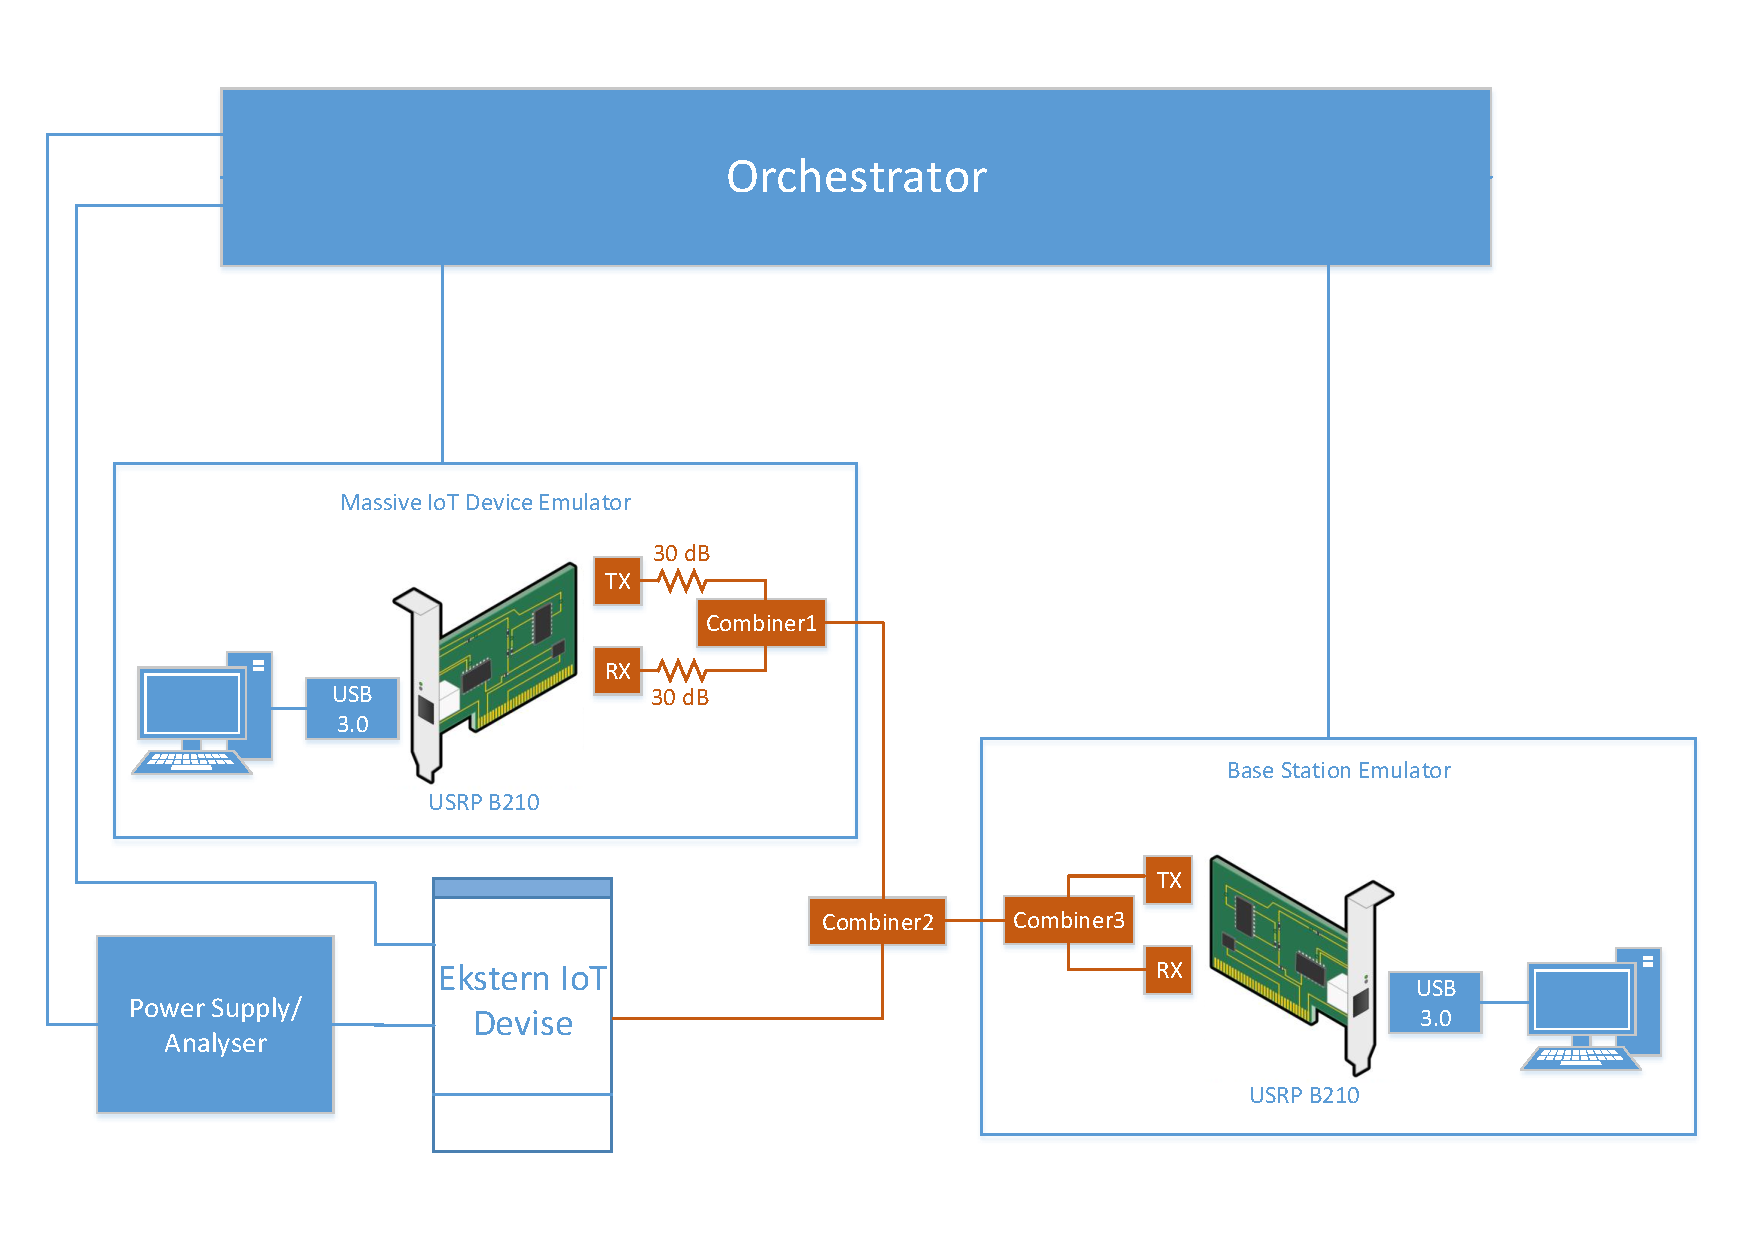
\includegraphics[width=\textwidth]{figures/General_test_setup.pdf}
\caption{A setup which enables testing of all domains on a single device through the massive device emulation.}
\label{fig:Fsetup}
\end{figure}


The setup contains the MDE for the massiveness domain, which will produce interference, both at a signaling level and sharing resources at different layers of the protocol. The PSU will provide power and analyze the power consumption for the DUT. The only domain not tested in this project is the reliability, this could be tested through logging of retransmissions. For this part emulation of different channel conditions for the DUT is very important, as reliability is severely affected by the channel. This is thought to be enough to measure each domain, as other parameters that affect the reliability are already built into the system, like the different cell parameters from the NB-IoT protocol.

